\section{Travaux réalisés}
\addetoc{section}{Completed works}
\paragraph{}
Mon stage consiste à mettre en \oe{}uvre un prototype de module de
spécialisation de code LLVM pour backend OpenCL de la chaîne de compilation
présentée plus haut. Autrement dit la passe LLVM qui se charge de transformer le
code en LLVM IR étendue du frontend R vers un code IR pur pour tout périphérique
supportant l'OpenCL. Il me faut donc commencer par connaître le modèle de
programmation OpenCL.

\subsection{OpenCL}
\addetoc{subsection}{OpenCL}
\subsubsection{Modéle de programmation OpenCL}
\addetoc{subsubsection}{OpenCL programming model}
\paragraph{}
OpenCL (Open Computing Language) est un standard de programmation proposé par le
\emph{Khronos group}~\cite{opencl} qui offre au développeur un moyen de
programmation parallèle hétérogène permettant de cibler les différentes
architectures de la machine, un code OpenCL peut donc tout aussi bien être
exécuté sur un CPU multi-c\oe{}urs que sur un accélérateur massivement parallèle
tels que les GPUs et le Xeon Phi.

Il offre donc une autre manière de programmer en faisant une distinction entre
le code hôte qui est exécuté par le CPU et qui fait appel au noyau de calcul
(\emph{kernel} en anglais) qui est compilé et adapté pour le périphérique de
calcul choisi. Le \emph{kernel} est écrit en OpenCL C, une combinaison d'une API
et du langage C. Le \emph{kernel} est exécuté par chaque \emph{thread} OpenCL ou
\emph{work-item} qui sont organisés en blocs \emph{work-group} qui sont
eux-mêmes regroupés dans une grille \emph{NDRange}.

La grille et les blocs peuvent être découpés en plusieurs dimensions, allant de
1 à \og{} CL\_DEVICE\_MAX\_WORK\_ITEM\_DIMENSIONS \fg{} qui dépend du
périphérique de calcul choisi ; la dimension est donnée lors du lancement du
\emph{kernel} au même moment que les tailles de ces derniers. On pourra ensuite
dans le \emph{kernel} récupérer ces informations ainsi que l'ID local au sein
d'un work-group ou global dans la NDRange du \emph{thread} en cours d'exécution
afin de potentiellement définir une instruction spécifique qu'à une certaine
partie des \emph{threads}. Néanmoins, les \emph{threads} sont exécutés par
paquet, en fonction de la taille de l'unité vectorielle du périphérique, un
paquet de work-item est exécuté en parallèle, il est donc préférable d'y tenir
compte lors de la définition des tailles de bloc et de l'écriture du
\emph{kernel}. Il faut aussi faire attention à ne pas dépasser la taille
maximale d'un bloc ou de la grille pour chaque dimension : elle dépend du
périphérique utilisé et peut être récupérée grâce à des fonctions OpenCL dans le
code hôte.

Il existe plusieurs types de mémoires en OpenCL selon le niveau dans la
hiérarchie, chaque work-item possède une mémoire privée. Les work-items d'un
même work-group se partagent une mémoire locale, et puis tous les work-items de
tous les work-groups ont accès à une mémoire globale et une mémoire constante.
Chacune de ces mémoires a une vitesse d'accès dépendant de leur localité par
exemple les \emph{threads} d'un même bloc accéderont plus rapidement à la
mémoire locale qu'à la mémoire globale.

Un périphérique OpenCL peut contenir une ou plusieurs unités de calcul (compute
units), un work-group est exécuté sur une seule unité de clacul qui contient une
mémoire locale.\\
La figure~\ref{opencl_memory_model} schématise ce qui a été dit.

\begin{figure}[h]
   \begin{center}
      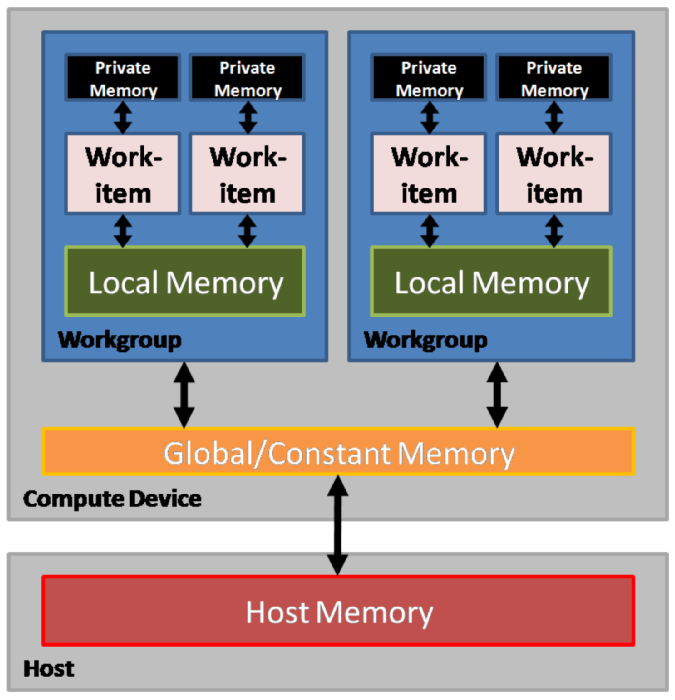
\includegraphics[scale=0.25]{./images/opencl_memory_model.png}
   \end{center}
   \caption{Modèle de mémoire OpenCL~\cite{opencl_memory_model}}
   \label{opencl_memory_model}
\end{figure}

\subsubsection{SPIR}
\addetoc{subsubsection}{SPIR}
\paragraph{}
Le \emph{kernel} est généré après une passe de spécialisation OpenCL de LLVM, il
est écrit en \emph{SPIR}~\cite{spir}, un langage bas niveau, qui fait la
correspondance entre OpenCL et le langage LLVM. Les versions 1.2 et 2.0 sont
d'ailleurs basées sur ce dernier. Il adopte deux des trois formats de
représentation de LLVM : le bitcode et l'assembleur. Il est supporté par tous
les périphériques utilisant OpenCL et chargeant l'extension \og{} khr\_spir
\fg{}.

Le mangling~\cite{spir_mangling} (création de symbole) des fonctions se base sur
le type des arguments de cette fonction, il adopte les concepts de l'ABI Itanium
C++. Par exemple, le symbole correspondant en SPIR de la fonction $\sin$(float),
est $\_Z3sinf$.

\subsection{Adaptation du runtime}
\addetoc{subsection}{Runtime adaptation}
\paragraph{}
Une fois la prise en main du modèle de programmation OpenCL, il me fallait
intégrer les fonctions de chargement de plateforme et de périphérique de calcul
et les appels de lancement de \emph{kernel} au runtime de \emph{Mach}. La
première partie est gérée par StarPU à l'initialisation du programme tout comme
la gestion de mémoire. Des fonctions permettent par la suite de récupérer leurs
identifiants qui sont stockés dans des structures spécifiques. Il fournit aussi
des fonctions de chargement et compilation de programme à partir de fichier
écrit en OpenCL C, ou d'un binaire déjà compilé par lui-même placé dans un
dossier temporaire qu'il aura créé durant l'exécution, dépendant du périphérique
utilisé et d'autres informations, ainsi qu'une fonction de chargement des
\emph{kernels} qu'il contient.\\
Néanmoins, nous voulons charger un binaire qui n'a pas déjà été compilé par
StarPU, et par conséquent dont il n'a pas défini l'emplacement ; ainsi pour
éviter de modifier le code source de cette dernière, je dois réimplémenter cette
fonction dans notre runtime, en gardant les même structures de stockage pour le
programme et les \emph{kernels}, de plus un oubli de libération de fichier s'est
glissé dans le code de cette fonction, ce qui cause une surcharge des registres
au bout d'un certain nombre de fichiers ouverts, ça me permet en même temps de
remédier à cette erreur.

À l'initialisation, StarPU scanne la machine afin de détecter les plateformes
et périphériques supportant OpenCL. Par défaut il ne recherche que les GPUs et
accélérateurs type Xeon Phi, et privilégie les GPUs. Étant donné que certains
GPU Nvidia ne supportent pas le SPIR, le programme plantera à l'exécution, j'ai
donc ajouté une variable d'environnement qui permet de désactiver la recherche
de GPU.

Les tableaux passés en arguments au \emph{kernel} OpenCL, doivent être des
handles sur ces dernier, c'est-à-dire, qu'on doit passer un pointeur sur la
première case. Les ND array sont généralement des vues, le premier élément ne se
trouve donc peut-être pas à la première case du tableau. Contrairement à la
passe de spécialisation Cuda le décalage doit être effectué dans le
\emph{kernel}. J'ai modifier le \emph{scratchpad} pour enregistrer l'indice du
premier élément de chaque ND array, que je récupère ensuite à l'aide d'une
fonction que j'ai implémenté dans le \emph{kernel} et je place le pointeur au
bon endroit.

\subsection{SPIR-Tools}
\addetoc{subsection}{SPIR-Tools}
\paragraph{}
Avant de commencer la spécialisation de code par passe LLVM, j'ai dû d'abord
prendre en main le langage SPIR et vérifier que le runtime StarPU gère bien ce
dernier, j'ai utilisé pour cela un outil fourni par le Khronos
group~\cite{spir_clang} qui s'intègre au compilateur clang permettant la
génération du binaire en SPIR à partir d'un \emph{kernel} écrit en OpenCL C.
J'ai donc écrit la version OpenCL du calcul de \emph{jacobi}, l'un des cas
utilisateur implémenté pour nos tests, qui fait la somme de chaque élément $(i,
j)$ avec ses voisins $(i+1, j)$, $(i-1, j)$, $(i, j+1)$, $(i, j-1)$, ces deux
derniers sont pondérés par un coefficient K, le tout multiplié par un réel R.
\[ B(i, j) = R * ( k*k * A(i, j-1) + k*k * A(i, j+1) + A(i-1, j) + A(i+1, j)) \]
Le calcul est suivi d'une opération de réduction pour le comparer au seuil de
convergence.

Tout en respectant le concept de programmation OpenCL, le calcul écrit est donc
celui exécuté par chaque \emph{thread}. La manière la plus simple de l'écrire
est donc de laisser chaque \emph{thread} s'occuper d'un élément. Cette version
du \emph{kernel} est bien évidemment d'abord testée avant de passer à la version
binaire en SPIR. En faisant appel à la fonction StarPU qui permet de lire les
fichier écrits en OpenCL C et de le compiler.

On récupère l'ID global d'un \emph{thread} avec la fonction
\emph{get\_global\_id(uint dimindx)}, avec dimindx la dimension sur laquelle on
souhaite l'avoir. Le code correspondant est en figure~\ref{jacobi_calc_ocl_kernel}.

\lstset{
   frame=L,
   language=c,
   keywordstyle=\color{blue},
   basicstyle=\footnotesize,
   breaklines=true,
   breakatwhitespace=false,
}
\begin{figure}[h]
   \lstinputlisting{./code/tf_opencl_kernel.cl}
   \caption{Calcul de Jacobi en OpenCL C}
   \label{jacobi_calc_ocl_kernel}
\end{figure}

On souhaite maintenant convertir ce \emph{kernel} OpenCL C en SPIR. On lance
alors la compilation du \emph{kernel} avec clang, puis on passe le fichier
généré en argument de la fonction implémentée dans notre runtime qui lit les
fichiers binaires. Le test passe parfaitement, le \emph{kernel} est chargé et
exécuté par notre programme sur les plateformes de calcul Intel (CPU et KNC Xeon
Phi), la carte GPU Nvidia quant à elle ne possède pas l'extension khr\_spir et
ne peut donc pas exécuter notre \emph{kernel}.

On peut visualiser la version assembleur de ce code SPIR grâce à la commande
\emph{llvm-dis}~\cite{llvm_cmd} qui permet de désassembler un fichier binaire.
Cela nous permet de voir la génération d'un code SPIR correct. On peut
appercevoir les métadonnées ajoutées en fin de fichier qui fournissent des
informations complémentaires à la compilation ; la spécification d'adress space
pour les pointeurs passés en arguments de la fonction, et le mangling des
fonctions \emph{kernel} utile à la récupération de l'ID du \emph{thread}.\\
La figure~\ref{jacobi_calc_spir_kernel} montre le code de calcul en SPIR généré,
sur lequel j'ai appliqué quelques modifications d'optimisations, telles que le
réarrangement des opérations arithmétiques pour éviter la redondance de calcul
ou de conversion de type.

\clearpage
\lstset{
   frame=L,
   language=llvm,
   keywordstyle=\color{blue},
   basicstyle=\tiny,
   breaklines=true,
   breakatwhitespace=false,
}
\begin{figure}[h!]
   \lstinputlisting{./code/tf_opencl_kernel.ll}
   \caption{Calcul de Jacobi en SPIR}
   \label{jacobi_calc_spir_kernel}
\end{figure}
\clearpage

Le tableau~\ref{spir_mangling} résume certaines fonctions OpenCL de récupération
d'informations sur le \emph{thread} courant et leur symbole SPIR correspondant.

\begin{table}[h]
   \begin{center}
      \begin{tabular}{|c|c|}
         \hline
         OpenCL C & Spir symbol \\
         \hline
         get\_global\_id & \_Z13get\_global\_idj \\
         \hline
         get\_global\_size & \_Z15get\_global\_sizej \\
         \hline
         get\_local\_id & \_Z12get\_local\_idj \\
         \hline
         get\_local\_size & \_Z14get\_local\_sizej \\
         \hline
         get\_work\_dim & \_Z12get\_work\_dim \\
         \hline
         get\_num\_groups & \_Z14get\_num\_groupsj \\
         \hline
         get\_group\_id & \_Z12get\_group\_idj \\
         \hline
         barrier & \_Z7barrierj \\
         \hline
      \end{tabular}
   \end{center}
   \caption{Correspondance entre la fonction OpenCL et son symbole Spir}
   \label{spir_mangling}
\end{table}

\subsection{Spécialisateur}
\addetoc{subsection}{Specializer}
\paragraph{}
La spécialisation de code est une opération de transformation du code LLVM IR,
ce qui revient donc à effectuer une passe dans LLVM~\cite{llvm_pass}.

L'exécution d'un programme OpenCL se fait par l'appel du CPU au \emph{kernel},
le spécialisateur prend donc en entrée un module et en fournie deux : un pour
le code SPIR et un pour le code hôte qui fera appel aux \emph{kernels} du
premier module.

\subsubsection{Code hôte}
\addetoc{subsubsection}{Host code}
\paragraph{}
J'ai maintenant compris comment créer un module LLVM et faire appel à des
fonctions, ajout de variable globale, etc.\\
J'ai aussi pris en main le modèle des passes déjà existante, sur lesquelles je
base mon travail pour garder une uniformité dans l'architecture logicielle.

Je commence par générer la partie hôte du code. Je suppose que le code
\emph{kernel} existe déjà, j'utilise le fichier SPIR créé précédemment, et je
fait les appels de fonction nécessaires au chargement et à la compilation du
programme, puis à la fonction de chargement du \emph{kernel} à partir de ce
programme, et je l'exécute grâce aux fonctions implémentées dans notre runtime.

Le fait de compiler le programme à chaque appel de tâche crée un goulot
d'étranglement qui ralentit énormément le programme et empêche le scheduler de
tirer profit au maximum des performances du matériel utilisé. Nous verrons par
la suite la solution employée pour contourner ce problème.

La première étape est de donner les paramètres de notre kernel à OpenCL, nous
devons lui passer les pointeurs vers ceux-ci sous la forme d’un tableau, on
l'appellera opération de packing d’argument. Ensuite la fonction
appelle \emph{setup\_ocl\_program()} et \emph{setup\_ocl\_kernel()}, deux
fonctions que j’ai écrites. La première récupère un handle sur le programme à
partir d'une chaînes de caractères contenant le nom du fichier à charger ; la
deuxième renvoie un handle sur le \emph{kernel} à partir du handle sur le
programme et d'une chaîne de caractères pour le nom du kernel. Pour connaitre le
nombre de blocs à utiliser, la taille de l’un des ND arrays est récupérée (on
suppose qu’ils sont de même taille) et divisée par le nombre de \emph{threads},
puis on boucle sur le nombre de dimension $-1$ que l'on choisi pour diviser les
blocs et la grille, et on calcul la racine carrée du nombre de blocs et de
\emph{threads}, qui représentent les nouvelles tailles de chaque dimension, pour
les passer en arguments de la fonction de lancement du \emph{kernel}.

Je passe maintenant à la génération du module \emph{kernel} sous les trois types
de tâches possibles.  Cette information est contenue dans une métadonnée qui est
lue par le code hôte et résidant uniquement en mémoire CPU.

\subsubsection{Ufunc}
\addetoc{subsubsection}{Ufunc}
\paragraph{}
Comme cité dans la section~\ref{particular_function}, une ufunc est une fonction
qui s'applique élément par élément ce qui rend l'utilisation des ALV facile,
étant donné que les opérations sur les vecteurs dans LLVM s'effectuent
principalement élément par élément. On passe le code au spécialisateur sous
cette forme vectorielle.

Les ufunc sont alors adaptées en tâches, dont les arguments sont les ND array
d'entrée et de sortie et d'autres valeurs selon la tâche.

Dans un premier temps les ND array sont chargés dans des ALV, à l'aide de
fonctions implémentées dans le runtime. On effectue les opérations voulues sur
ces ALV, puis on enregistre l’ALV résultant dans un ND array.

\subsubsection{Rfunc}
\addetoc{subsubsection}{Rfunc}
\paragraph{}
Une rfunc est une opération de réduction de vecteurs, le passage d'une dimension
à $n$ éléments à 1 élément contenant la somme, le maximum ou le minimum de tous
ces éléments.

Je me suis basé pour la réduction parallèle sur l'algorithme et les différentes
optimisations présentées par \emph{AMD}~\cite{ocl_reduction}, et des
optimisations effectuées dans la passe Cuda qui se sont avérées performantes sur
les GPU Nvidia.

Le principe est d'effectuer une réduction binaire. On attribue à chaque
\emph{thread} un élément du vecteur qui lit cette valeur et l'enregistre dans
une case d'un tableau en mémoire locale, déclarée au préalable, de taille égale
au nombre de \emph{threads} par bloc (j'ai expliqué plus haut que les work-items
d'un même work-group se partagent une mémoire locale plus rapide d'accès). La
réduction se fait ensuite sur ce tableau, on considère que seule la première
moitié des \emph{threads} sont actifs. Chacun fait la réduction de deux valeurs
$i$ et $(i+n/2)$, $n$ étant la taille du tableau et l'enregistre dans la case
qui lui est affectée. À l'itération suivante, le nombre de \emph{threads} actifs
est divisé par deux ainsi que la taille théorique du tableau partagé. Le pas de
décalage pour la deuxième valeur à additionner n'est plus $n/2$ mais $n/4$. Et
ainsi de suite jusqu'à ce qu'il ne reste qu'un \emph{thread} actif qu'on
considérera comme étant le \emph{thread} maître, comme dans la
figure~\ref{binary_sum}. Ce dernier enregistre le résultat en mémoire globale
dans le \emph{scratchpad} (notre vecteur particulier initialisé avant le
\emph{kernel}).

\begin{figure}[h]
   \begin{center}
      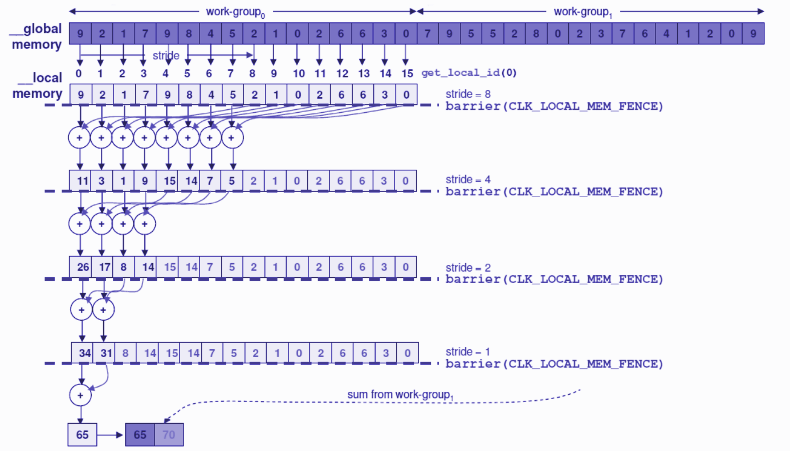
\includegraphics[scale=0.75]{./images/binary_reduce.png}
   \end{center}
   \caption{Réduction binaire en mémoire locale~\cite{binary_sum}}
   \label{binary_sum}
\end{figure}

Une fois la réduction terminée par tous les blocs on retrouve nos résultats de
réduction partielle en mémoire globale ; on relance alors le \emph{kernel} avec un
nombre de \emph{threads} égal au nombre de blocs du \emph{kernel} précédent, afin de
faire la dernière réduction sur un bloc.\\
Néanmoins le nombre de \emph{threads} par bloc étant limité, dans le cas d'un
très grand vecteur d'entrée, le nombre de résultats partiels au premier
lancement de \emph{kernel} pourrait dépasser cette limite, il faudrait alors
exécuter le \emph{kernel} autant de fois que nécessaire pour terminer la
réduction en un bloc.

Une autre solution plus performante inspirée de la passe Cuda est de modifier la
boucle de chargement des données en mémoire locale pour qu'elle fasse un nombre
d'itérations dépendant de la taille du vecteur. Cela permet d'avoir un nombre
fixe de blocs et donc de résultats partiels tout en sommant l'intégralité du
vecteur. On peut maintenant écrire la réduction en deux étapes.

\subsubsection{Sfunc}
\addetoc{subsubsection}{Sfunc}
\paragraph{}
Les sfunc sont des opérations de réduction cumulative sur un vecteur,
c'est-à-dire, que le résultat de réduction à l'itération $i$ est la réduction du
résultat précédent de l'itération $i-1$ et la valeur à l'indice $i$.

Comme pour les tâches précédentes, je me base pour l'implémentation de
l'algorithme parallèle sur la passe Cuda, en plus de quelques recherches en
ligne sur le sujet. Les étapes de la réduction parallèle se résume ainsi :
\begin{itemize}
   \item Faire une réduction binaire de deux éléments consécutifs.
   \item Faire le calcul récursif sur le résultat de la séquence précédente.
   \item Exprimer chaque terme de la séquence finale, comme la réduction de deux
      termes de ces séquences intermédiaires. Après la première valeur, les deux
      éléments de réduction sont l'élément $i$ et l'élément de la séquence
      précédente à l'indice $i+k/2$ (avec $k$ le pas entre deux élément de la
      séquence) et ainsi de suite jusqu'à arriver à la réduction des éléments de
      la séquence initiale.
\end{itemize}

\begin{figure}[h]
   \begin{center}
      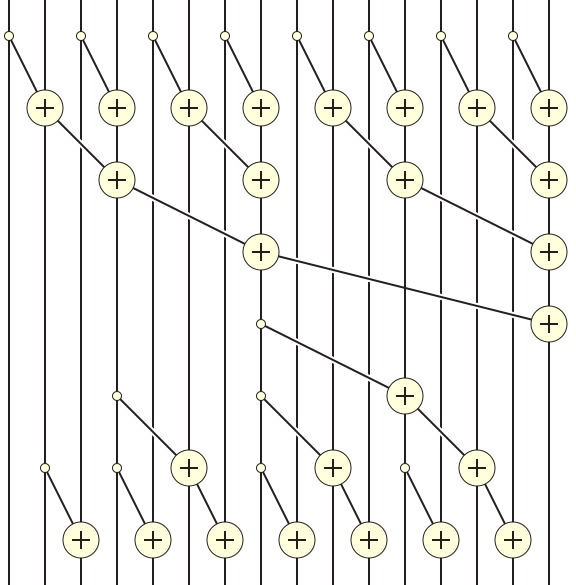
\includegraphics[scale=0.3]{./images/prefix_sum.png}
   \end{center}
   \caption{Somme cumulative parallèle~\cite{prefix_sum}}
   \label{prefix_sum}
\end{figure}

\subsubsection{Création de symbole SPIR OpenCL}
\addetoc{subsubsection}{Mangling fuction}
\paragraph{}
Les fonctions mathématiques usuelles telles que $\cos$ et $\sin$ sont nécessaires
au calcul scientifique. Mais ces fonctions ne correspondent pas à des
instructions disponibles sur le matériel, il est donc nécessaire de créer leur
symbole SPIR dans le \emph{kernel}. J'ai utilisé pour cela un outil fourni avec
le générateur de code SPIR du \emph{KHRONOS group}, que j'ai intégré au
spécialisateur OpenCL. Il suffit alors de remplacer les appels de fonctions
mathématiques par des appels aux fonctions avec le symbole correspondant.

\lstset{
   frame=L,
   language=llvm,
   keywordstyle=\color{blue},
   basicstyle=\footnotesize,
   breaklines=true,
   breakatwhitespace=false,
}
\begin{figure}[h!]
   \begin{subfigure}{135mm}
      \begin{lstlisting}
   %vnew = call <0 x float> @llvm.fabs.v0f32(<0 x float> %vold)
      \end{lstlisting}
      \caption{Intrinsèque LLVM de la fonction mathématique fabs}
   \end{subfigure}
   \\[5mm]
   \begin{subfigure}{135mm}
      \begin{lstlisting}
   %vnew = call float @_Z4fabsf(float %volv)
      \end{lstlisting}
      \caption{Symbole correspondant en SPIR de la fonction fabs}
   \end{subfigure}
\end{figure}

\subsection{Optimisation de compilation}
\addetoc{subsection}{Compilation optimization}
\paragraph{}
Je me suis basé sur une première optimisation de la passe Cuda pour le
chargement des données des ND array dans les ALV. Le principe est de passer au
module le nombre de dimension des ND array d'entrée/sortie. Le module va alors
créer quatre kernels : trois pour les dimensions classiques (1, 2 et 3) et un
pour toute les autres. Pour les ND array de dimension 1, 2 et 3, la variable est
remplacée par la constante correspondante ce qui permet au compilateur
d'effectuer des optimisations automatiques de déroulage de boucle ; quant aux
autres dimension la variable est chargée du \emph{scratchpad}.

Le plus gros ralentissement dans l'exécution du programme était bien évidemment
la compilation du programme OpenCL à chaque appel de la tâche, l'idéal est donc
de le charger une seuls fois à l'initialisation et de garder un pointeur dessus
pour y accéder si besoin.\\
Une passe d'initialisation existe déjà, elle se charge de créer la tâche adaptée
au runtime, c'est-à-dire, avec la signature correspondante et de transformer les
appels de fonctions en enregistrement et en soumission de tâches dans le main.

À la création de la tâche on fait donc appel à une fonction d'initialisation du
programme OpenCL, qui est compilé par notre fonction qui prend un fichier
binaire en entrée puis enregistre la structure retournée dans un tableau en
variable globale, référencé par l'index attribué au périphérique de calcul
détecté sur la machine sur lequel on l'a compilé. Cela nous permet de lancer
plus d'un worker en même temps sur des matériels différents de la machine, on
charge ensuite le \emph{kernel}, et dans le même cas que pour un programme, j'ai
réimplémenté la fonction de chargement du \emph{kernel}, et créé une
nouvelle structure semblable à celle utilisée pour le stockage du programme
compilé, dans laquelle on enregistre le \emph{kernel} en variable globale, j'ai
par conséquent aussi mis en place une fonction permettant de récupérer cette
donnée si besoin et une autre pour la libérer en fin d'exécution.

Une autre modification à faire : un programme OpenCL peut contenir plusieurs
\emph{kernels}, en quatre versions chacun, ce serait encore une fois une perte
de performance que de recompiler le programme sachant que c'est la phase la plus
contraignante lors du chargement de ce dernier. Il suffit alors pour éviter les
redondances de tester si la variable globale contenant le programme compilé est
nulle, et si elle ne l'est pas, de passer directement au chargement du
\emph{kernel}.

Le code de la figure~\ref{calc_jacobi} représente le calcul de jacobi en LLVM
IR. Le spécialisateur génère le code hôte et le code SPIR. La
figure~\ref{jacobi_task_create} montre le code de création de tâche et de
chargement du programme et du \emph{kernel} dans le code hôte.

\lstset{
   frame=L,
   language=llvm,
   keywordstyle=\color{blue},
   basicstyle=\tiny,
   breaklines=true,
   breakatwhitespace=false,
}
\begin{figure}[]
   \lstinputlisting{./code/tf_calc_next_val_task.ll}
   \caption{Tâche de calcul de jacobi en LLVM IR étendu}
   \label{calc_jacobi}
\end{figure}

\lstset{
   frame=L,
   language=llvm,
   keywordstyle=\color{blue},
   basicstyle=\tiny,
   breaklines=true,
   breakatwhitespace=false,
}
\begin{figure}[]
   \lstinputlisting{./code/jacobi_task_create.ocl.ll}
   \caption{Création de tâche et chargement du \emph{kernel} dans le code hôte}
   \label{jacobi_task_create}
\end{figure}
\clearpage

\subsection{Tests expérimentaux}
\addetoc{subsection}{Experimental tests}
\subsubsection{Description de la machine}
\addetoc{subsubsection}{Machine description}
\paragraph{}
J'ai effectué mes tests de spécialisation de code sur une machine équipée d'un
microprocesseur Intel Xeon E5-2620 2.00GHz, et d'un accélérateur Intel Xeon Phi
Coprocessor x100. C'est un KNC, disposant de 8 Go de RAM, 60 c\oe{}urs
multithreadés qui nous font 240 processeurs logiques avec une fréquence de base
de 1.053 GHz, et une bande passante théorique de 320 Go/s.

\subsubsection{Jacobi}
\addetoc{subsubsection}{Jacobi}
\paragraph{}
Je continue de tester le résultat obtenu de ma passe de spécialisation OpenCL
sur l'exemple de jacobi ; et je peux, maintenant, que j'ai implémenté toute les
fonctions nécessaires à la spécialisation des différents types de tâche, créer un
binaire contenant uniquement le code spécialisé qui tournera sur une plateforme
de calcul OpenCL. La passe crée un module pour le code hôte qui s'exécute sur le
CPU, crée les buffers sur le périphérique de calcul choisi et copie les
données dans ces derniers puis lance l'exécution du \emph{kernel}, et un autre
pour le code de calcul en SPIR.

J'ai testé l'exécution du noyau de calcul sur le CPU et le KNC, mais pas les
deux en même temps, car il y a deux versions de librairies OpenCL installées sur
la machine, la première ne gère que les matériel de type CPU et l'autre est
spécifique au Xoen Phi.

J'ai validé les résultats en les comparant à des fichiers de références des
spécialisateurs x86 et Cuda, qui ont tout deux été validés auparavant avec des
versions du code écrits à la main.

La commande \emph{htop} permet de voir la charge de travail sur la machine. J'ai
aussi utilisé le panneau de contrôle du Xeon Phi qui permet de voir la charge,
la mémoire consommée et la puissance exploité sur ce dernier. Des variables
d'environnement sur StarPU permettent aussi d'afficher des informations sur les
workers (temps et matériel d'exécution du programme). La figure~\ref{micsmc_gui}
montre le résultat pour une exécution, sur des tableaux de float de tailles
16386x8192, une tolérance de convergence de $10^{-3}$, et des bloc de 256
\emph{threads}.

\begin{figure}[h]
   \begin{center}
      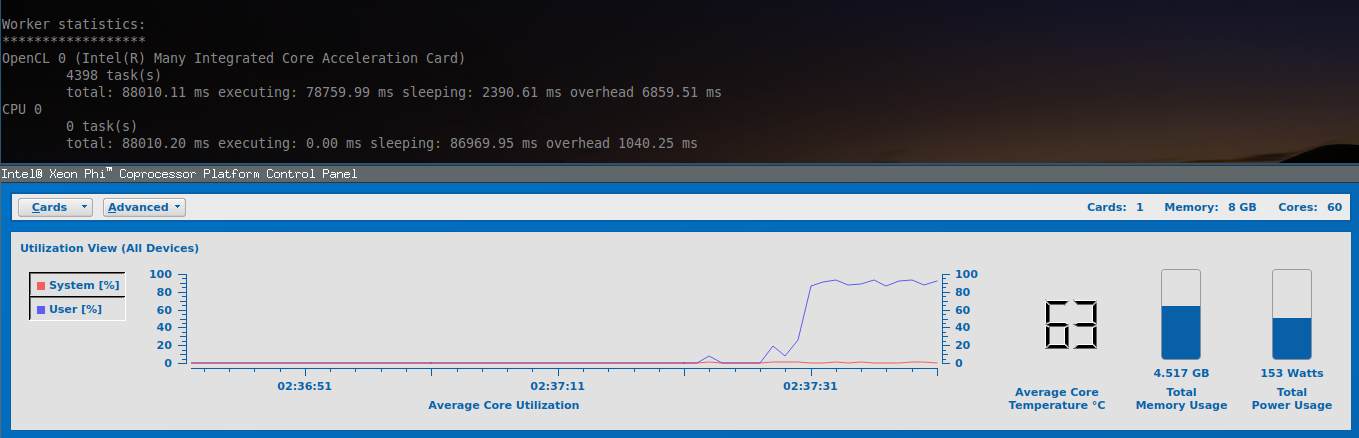
\includegraphics[scale=0.25]{./images/micsmc_gui.png}
   \end{center}
   \caption{Panneau de contrôle du Xeon Phi}
   \label{micsmc_gui}
\end{figure}

Les résultats semblent prometteurs mais un peut lent, on tire bien profit de la
puissance du matériel, mais l'exécution n'est pas assez fluide. J'utilise alors
un autre outil : \emph{Intel VTune} qui permet d'analyser le code, de voir le
code assembleur et vérifier que le compilateur a bien vectorisé les opérations
vectorielles, et d'afficher les point chaud qui font ralentir l'exécution. Il
apparaît que le problème vient du scheduler de tâches, ce dernier ne semble pas
tirer profit au maximum du matériel, le temps passé à attendre l'exécution
d'une tâche est trop grand par rapport au temps de calcul. J'ai tenté de changer
le nombre de \emph{threads} par bloc, pour essayer de lancer des paquets de
tailles multiple au nombre de c\oe{}urs ; certaines tailles montrées quelque
amélioration mais assez minime. Une analyse plus approfondie relèverais
peut-être de meilleure modification sans doute la modification de l'algorithme
ou du modèle d'exécution des tâches.

\subsubsection{Test de toute la chaîne de compilation}
\addetoc{subsubsection}{Test entire toolchain}
\paragraph{}
Le projet \emph{Mach} arrive bientôt à sa finalisation, la chaîne d'outils est
alors bien assez complète pour la tester entièrement en partant d'un code écrit
en \emph{K} représenté dans la figure~\ref{mandel_k}. C'est un code de calcul de
recherche des points appartenant à \emph{l'ensemble de mandelbrot}. Je le
compile à l'aide du frontend \emph{KFE}, qui génère deux fichiers en LLVM IR
étendue avec les notions d'ALV, ND array, etc. Le premier contient la fonction
\emph{main}, et l'autre les tâches de calcul. Je passe ces deux derniers au
spécialisateur OpenCL, qui génère à son tour les codes \emph{kernel} et le code
hôte. Le tout est ensuite compilé pour créer finalement un binaire pour
plateforme OpenCL.

\lstset{
   frame=L,
   language=c,
   keywordstyle=\color{blue},
   otherkeywords={*,call},
   basicstyle=\footnotesize,
   breaklines=true,
   breakatwhitespace=false,
}
\begin{figure}[h!]
   \lstinputlisting{./code/mandel.k}
   \caption{Mandelbrot écrit en K}
   \label{mandel_k}
\end{figure}
